% !TeX root=../../../main.tex

\chapter{مبانی تحقیق}
% دستور زیر باعث عدم‌نمایش شماره صفحه در اولین صفحهٔ این فصل می‌شود.
%\thispagestyle{empty}

در این فصل ابتدا مفاهیم مورد نیاز جهت تعریف مسئله مانند مدل¬های ناهمگنی تومور،‌ روش¬های یافتن درخت تکاملی تومور، روش¬های توالی¬یابی داده مورد بررسی قرار می¬گیرند. در ادامه مدل¬های مورد استفاده برای استنباط درخت تکاملی تومور معرفی می¬شوند. در پایان مفاهیم مرتبط با یادگیری ماشینی، یادگیری عمیق و یادگیری تقویتی به منظور استنباط درخت تکاملی تومور با \gls{datadriven}  توضیح داده می¬شوند.


\section{تنوع ژنتیکی}

\gls{dna}  یک مولکول بیولوژیکی است که توسط \glspl{nucleotid}  پلیمری شده است. در دی‌ان‌ای چهار نوع نوکلئوتید وجود دارد: \gls{adenine}  (A) ، \gls{thymine}  (T) ، \gls{cytosine}  (C) و \gls{guanine}  .(G) دی‌ان‌ای اساس توالی اسیدهای آمینه است که پروتئین را تشکیل می‌دهد. یک مولکول دی‌ان‌ای از دو رشته تشکیل شده است. که در \glspl{antiparallel}  هم و درجهت¬های مخالف قرار دارند و ساختاری از مارپیچ دوتایی ایجاد می‌کنند. هر نوع نوکلئوتید روی یک رشته با نوع دیگری از نوکلئوتید در رشته دیگر مرتبط است: A با T ؛ C با G (شکل \ref{fig:ch_lr:DNA_double_helix}) \cite{alberts2002molecular}. این به عنوان قانون پایه جفت شدن نوکلئوتید¬ها در هر رشته از دی¬ان¬ای شناخته می‌شود.


\begin{figure}[!ht]
	\centerline{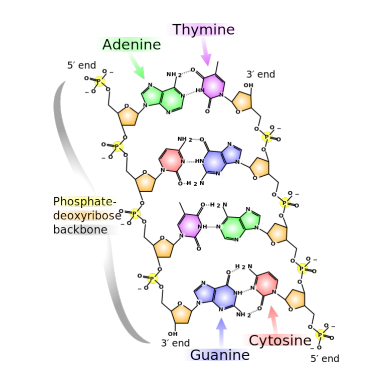
\includegraphics[width=11cm]{chaps/lr/DNA_double_helix}}
	\caption{مارپیچ دوگانه دی‌ان‌ای}
	\label{fig:ch_lr:DNA_double_helix}
\end{figure}



همانند سازی دی‌ان‌ای فرآیند تولید دو مولکول دی‌ان‌ای یکسان از مولکول دی‌ان‌ای اصلی است. وقتی تکثیر شروع می¬شود، دو رشته یک مولکول دی‌ان‌ای از یکدیگر جدا می¬شوند و هر رشته به عنوان الگویی برای ساخت نمونه مشابه خود عمل می‌کند. نوکلئوتید¬ها در هر موقعیت از یک رشته با نوع دیگری از نوکلئوتید مبتنی بر قانون پایه جفت شدن، به منظور سنتز همتای این رشته، متصل می‌شود. پس از همانند سازی ، مولکول دی‌ان‌ای اصلی به دو مولکول یکسان تبدیل می¬شود (شکل \ref{fig:ch_lr:DNA_replication}) \cite{alberts2002molecular}.

\begin{figure}[!ht]
	\centerline{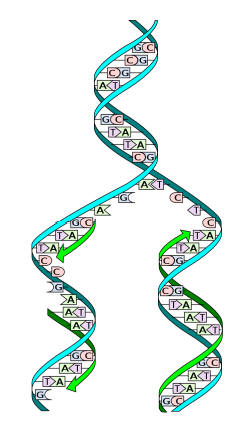
\includegraphics[width=8cm]{chaps/lr/DNA_replication}}
	\caption{همانندسازی دی‌ان‌ای}
	\label{fig:ch_lr:DNA_replication}
\end{figure}





ژن ناحیه¬ای از دی¬ان¬ای است و به عنوان مولکول واحد وراثت شناخته می¬شود. ژن¬های متعددی در ساختار دی¬ان¬ای با عملکرد¬های متفاوت وجود دارد. جهش به تغییر دائمی‌توالی هسته¬ای ژنوم اتلاق می¬شود. جهش¬ها می¬توانند در حین فرآیند تکثیر دی¬ان¬ای و با جفت¬گیری اشتباه در قسمت¬های مختلف دی¬ان¬ای ایجاد می¬شود. انواع مختلفی از جهش¬ها مانند \gls{snm}(\gls{pointmutation})  (شکل \ref{fig:ch_lr:single_nucleotide_mutation}) و  \glspl{singlevariant}  شامل \gls{insertion}  ، \gls{deletion}  و \gls{reversion}  (شکل \ref{fig:ch_lr:structural_changes}) وجود دارد. جهش¬های سلولی می¬توانند به بنا بر دلایلی چون مواد شیمیایی ، سمیت یا ویروس ایجاد شوند. جهش در یک ژن می‌تواند محصولات آن را تغییر دهد (مانند ایجاد پروتئین متفاوت) یا از عملکرد صحیح ژن جلوگیری کند \cite{alberts2002molecular}.




\begin{figure}[!ht]
	\centerline{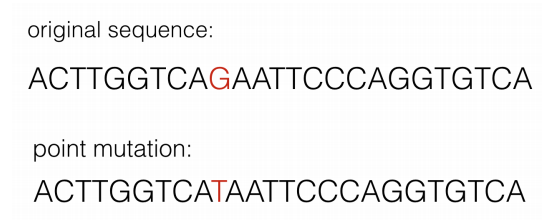
\includegraphics[width=10cm]{chaps/lr/single_nucleotide_mutation}}
	\caption{جهش تک‌نوکلئوتیدی}
	\label{fig:ch_lr:single_nucleotide_mutation}
\end{figure}



\begin{figure}[!ht]
	\centerline{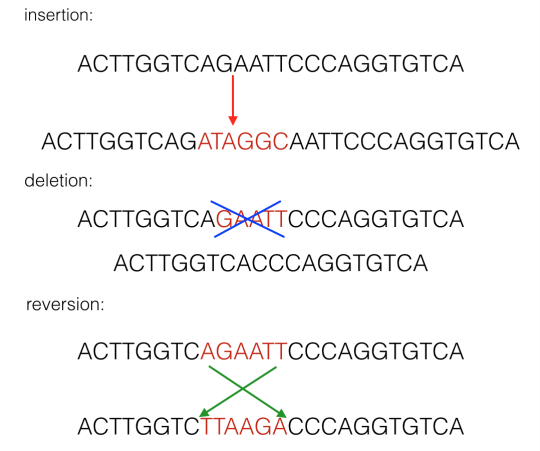
\includegraphics[width=10cm]{chaps/lr/structural_changes}}
	\caption{تغییرات ساختاری}
	\label{fig:ch_lr:structural_changes}
\end{figure}




\section{\gls{tumorevolution}}


جهشی که در هر سلول از بدن اتفاق می‌افتد، به استثنای سلول‌های جنسی (اسپرم و تخمک)، جهش \gls{somatic}  نامیده می-شود \cite{somaticMutation}. تجمع جهش بدنی در طول زندگی یک فرد می‌تواند منجر به رشد کنترل نشده مجموعه‌ای از سلول(تومور) شود \cite{nowell1976clonal} و می‌تواند باعث شکل¬گیری سرطان یا بیماری¬های دیگر شود \cite{somaticMutation}. بدلیل تجمع سلول‌های گوناگون، بیش از یک نوع سلول در تومور وجود خواهد داشت. به گروه¬های سلول با مجموعه‌ای از جهش مشخص ، کلون یا جمعیت سلولی تومور گفته می‌شود. کلون¬های موجود در تومور از نظر فیلوژنتیک با هم مرتبط هستند و رابطه آنها را می¬توان با یک درخت فیلوژنتیک نشان داد \cite{birbrair2014type}. درخت فیلوژنتیک رابطه تکاملی بین کلون و ترتیب وقوع هر جهش را نشان می‌دهد. به عنوان مثال ، شکل\ref{fig:ch_lr:tumor_phylogenetic_tree} :

\begin{itemize}
	\item یک درخت فیلوژنتیک از یک تومور با چهار کلون با برچسب 0 تا 3  را نشان می¬دهد.
	\item جهش جدیدی را نشان می¬دهد که در هر کلون در طول تکامل این تومور رخ داده است.
\end{itemize}

 همچنین هر کلون جهشی را در مسیر از کلون بالایی به سمت خود به ارث می‌برد. به عنوان مثال ، کلون 0 جهش¬های m0 ، m1 دارد. کلون 1 دارای جهش m0 ، m2 ، m3 ، m4 است.
 
\begin{figure}[!ht]
	\centerline{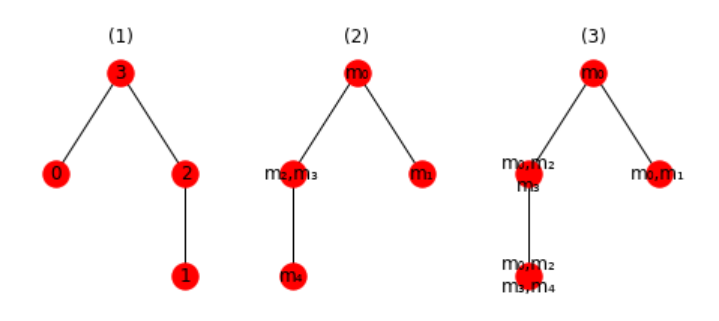
\includegraphics[width=10cm]{chaps/lr/tumor_phylogenetic_tree}}
	\caption{درخت فیلوژنیک تومور}
	\label{fig:ch_lr:tumor_phylogenetic_tree}
\end{figure}


\section{تکنولوژی¬های توالی¬یابی و \gls{variantallelefrequency}}




تعیین توالی دی‌ان‌ای روشی برای تشخیص ترتیب دقیق نوکلئوتیدها در یک رشته دی‌ان‌ای است. روش \gls{nextgenerationsequencing}  از تعدادی فناوری مدرن توالی تشکیل شده است که امکان تعیین هزینه و زمان توالی¬یابی را به طور موثر فراهم می-کند. با استفاده از نمونه بیولوژیکی به عنوان ورودی این تکنولوژی¬ها، توالی¬های کوتاه نوکلئوتیدی تولید می¬شود (که به آن \gls{read}  گفته می¬شود). سپس خوانش با استفاده از الگوریتم \gls{alignment}  متنوعی مانند الگوریتم تبدیل \lr{Burrows-Wheeler} با ژنوم مرجع تراز می‌شوند. پس از ترازبندی ، می‌توان با جمع‌آوری \glspl{overlappingread}،  توالی \gls{consensus}  ایجاد کرد (شکل \ref{fig:ch_lr:alignment_reading}). در موقعیتی از توالی اجماع به دلیل همپوشانی خوانش ها، ممکن است بیش از یک نوع خوانش از نوکلئوتید تراز شده وجود داشته باشد (تعداد کل قرائت مرتبط با یک نوع جهش، را \gls{readcoverage}  نامیده می¬شود). نوکلئوتید موجود در این موقعیت به عنوان رایج¬ترین نوکلئوتید تراز شده، مشخص می¬شود. به عنوان مثال، در شکل \ref{fig:ch_lr:alignment_reading} ، سه آدنین (A) ، یک گوانین (G) و یک تیمین (T)  در موقعیت سوم توالی اجماع تراز می‌شوند ، سپس نوکلئوتید در آن موقعیت به عنوان آدنین (A) تعیین می‌شود. پس از ایجاد توالی اجماع ، نوکلئوتیدهای موجود در آن توالی، که متفاوت از ژنوم مرجع هستند، شناسایی شده و به عنوان \gls{somaticsnv}  شناخته می¬شود. با استفاده از نمونه¬های متعدد استخراج شده از یک نمونه تومور، ما می‌توانیم تغییرات بدنی تک نوکلئوتیدی را در هر نمونه با فناوری تعیین توالی¬یابی تشخیص دهیم. نسبت تعداد سلول‌های موجود در یک نمونه حاوی تغییرات بدنی تک نوکلئوتیدی به کل سلول‌ها، فراوانی تغییرات آلل یک تغییر بدنی تک نوکلئوتیدی در این نمونه نامیده می¬شود. مقادیر فراوانی تغییرات آلل برای هر تغییر بدنی تک نوکلئوتیدی  در هر نمونه تومور قابل محاسبه است. ابزارهای زیادی برای بازسازی درخت فیلوژنتیک تومور از مقادیر فراوانی تغییرات آلل تومور به عنوان ورودی الگوریتم استفاده می¬کنند.



\begin{figure}[!ht]
	\centerline{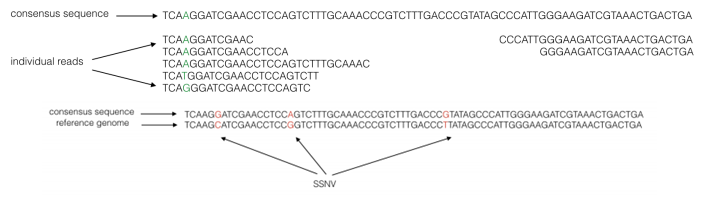
\includegraphics[width=\textwidth]{chaps/lr/alignment_reading}}
	\caption{تشخیص تغییر بدنی تک‌نوکلئوتیدی از طریق خوانش هم‌ترازی}
	\label{fig:ch_lr:alignment_reading}
\end{figure}



\section{ناهمگنی ژنومی تومور}


سرطان بیماری¬ای است که بدلیل ایجاد ناهنجاری¬های اساسی در فرآیند¬های بنیادی سلول مانند \gls{replication}\ ، \gls{differentiation}  و \gls{death} سلول  ایجاد می¬شود \cite{hanahan2011hallmarks}. این ناهنجاری منجر به رشد کنترل نشده تومور و به¬کارگیری بافت غیرسرطانی برای حمایت از این رشد می شود. علت اصلی این تغییرات جهش است. جهش یک اصطلاح گسترده است که چندین دسته از تغییرات ژنتیکی را پوشش می¬دهد. هنگام حاملگی ، یک جنین دارای یک ژنوم خاص و منحصر به فرد است. این ژنوم که به \gls{germlinegenome} معروف است، می¬تواند با ژنوم انسانی مرجع مقایسه شود. ژنوم انسانی مرجع یک نمونه از ژنوم انسان است و از دی‌ان‌ای چند نفر تشکیل شده است. تفاوت بین ژنوم جوانه‌زنی و ژنوم مرجع به عنوان جهش ژنوم جوانه زنی شناخته می-شود. جهش¬های جوانه زنی می¬توانند مسئول افزایش خطر ابتلا به سرطان باشند \cite{stewart2017world} ، اما بندرت خود مسئول مستقیم توسعه تومور هستند. 




معمولاً تومورها در اثر جهش¬های اکتساب شده پس از لقاح ، که معروف به جهش¬های بدنی هستند، ایجاد می شوند. جهش-های بدنی نتیجه اشتباهات در تکثیر دی‌ان‌ای \cite{behjati2014genome} ، قرار گرفتن در معرض جهش¬های با منشأ داخلی یا خارجی یا وارد¬شدن توالی¬های دی‌ان‌ای با منشأ بیرونی بدلیل قرار گرفتن در معرض ویروس است \cite{talbot2004viruses}. غالباً در سرطان ، جهش های بدنی باعث ایجاد اختلال در روند تکثیر دی‌ان‌ای یا ترمیم آن می شوند و حتی جهش های بدنی بیشتری ایجاد می کنند \cite{stratton2009cancer}. نظریه کلونی بودن سرطان \cite{nowell1976clonal} سرطان را به عنوان یک تک سلولی با منشأ غیرجنسی در نظر می¬گیرد که در اثر تولید مثل فراوان، یک توده متشکل از کلون¬های سلولی گوناگون را ایجاد می¬کند. در این مدل سلولهای توموری با یکدیگر در رقابت هستند و جهش¬های بدنی که مزیت رشد را ایجاد می کنند در جمعیت سلول¬های توموری از نسبت بیشتری برخوردار خواهند بود. جهش¬های بدنی که باعث رشد تومور شده و از سلولی به سلولی دیگر منتقل می¬شوند به عنوان \glspl{drivermutation} شناخته می¬شوند. اولین سلولی که دارای جهش راننده بوده و آن را به جهش¬های بعدی منتقل می¬کند به عنوان سلول بنیانگذار شناخته می شود. همه فرزندان این سلول بنیانگذار، جهش راننده و هر جهش دیگری را که سلول بنیانگذار قبل از به دست آوردن جهش راننده بدست آورده است، دارند. این جهش¬های دیگر ، که مزیتی برای رشد و گسترش تنوع توموری ندارند ، به عنوان \glspl{passengermutation} شناخته می¬شوند. شایان ذکر است که تعریف جهش راننده و مسافر به زمینه ژنتیکی و محیطی بستگی دارد. به عنوان مثال ، شیمی درمانی \gls{cytotoxic}  (سیتوتوکسیک) می تواند باعث تغییر جهش از مسافر به جهش راننده شود و عامل اصلی مقاومت در برابر درمان باشد. همچنین جهش ها را می توان بر اساس نوع تغییری که در دی‌ان‌ای ایجاد می شود ، به طبقات متمایز تقسیم کرد. \gls{snv} جهش¬هایی هستند که یک پایه در ژنوم را به پایه دیگری تغییر می دهند. \gls{indel}  درج یا حذف یک بخش دی‌ان‌ای است که می تواند کوتاه یا طولانی باشد. از ایندل کوتاه و تغییرات تک نوکلئوتیدی در مجموع به عنوان \glspl{ssm}  یاد می شود. در همه قسمت¬های یک ژنوم، از جمله کل کروموزوم¬ها، قابلیت حذف یا کپی شدن قسمتی از ژنوم وجود دارد. تغییرات شماره کپی  به جهشی اتلاق می¬شود که منجر به حذف یا کپی شدن قسمتی از ژنوم می¬شود. \gls{cna} نوعی \gls{singlevariant} هستند که شامل وارونگی (وقتی قسمت بزرگی از ژنوم معکوس شده باشد) و انتقال متعادل (جایی که دو بخش ژنومی مکان¬¬های خود را با یکدیگر تعویض می¬کنند) می¬باشند\cite{stratton2009cancer}. این گونه¬های مختلف جهش مستقل از یکدیگر نیستند و می توانند در رابطه با یکدیگر اتفاق بیفتند (به عنوان مثال یک جهش می¬تواند منجر به تقویت یک وارونگی شود). 



تکنیک توالی¬یابی نسل بعدی این امکان را فراهم کرده است تا با صرف هزینه بسیار کم و با استفاده از یک نمونه توموری، توالی¬یابی از دی¬ان¬ای صورت پذیرد و همین امر منجر به تحول گسترده¬ای در زمینه مطالعه تکامل تومور شده زیر امکان نمونه-برداری در تعداد بسیار بالا را از تومور فراهم می¬کند. نمونه¬گیری در حجم بالا این امکان را فراهم آورده است تا ناهمگنی تومور از نقطه منظر ژنتیکی مورد بررسی قرار گیرد و پاسخ به درمان بیماران سرطانی با جزییات بیشتری مورد ارزیابی قرار گیرد.


تقریباً همه نمونه¬های استخراج شده از تومور ترکیبی از سلول ها با ژنوتیپ¬های مختلف را شامل می¬شود. یک نمونه توموری به ندرت فقط شامل بافت سرطانی است زیرا شامل سلول های غیر سرطانی از \gls{surroundingstroma}  یا \glspl{Infiltratingimmunecell}  است. مطالعات ژنومیک نشان داده است که حتی در میان سلولهای سرطانی، غالباً زیرجمعیت¬های متعدد سرطانی نیز وجود دارد. به عنوان مثال ، در یک مطالعه مهم در سال 2012 ، گرلینگر و همکارانش \cite{gerlinger2012intratumor} توالی¬یابی ژنوم و تغییرات شماره کپی را از طریق نمونه¬های مکانی مجزا استخراج شده از سرطان کلیه اولیه و نقاط متاستاز ثانویه بدست آورده¬اند. با بررسی  این نمونه¬های متعدد ، مشخص شد که یک ناهمگنی ژنتیکی قابل توجهی در تومور وجود دارد. تعداد بسیار زیادی از جهش¬های شناسایی شده در همه سلول¬های توموری مشاهده نشدند و این بدان معناست که این جهش¬ها بیش از آن¬که یک ناحیه کلونی باشند، به صورت یک ناحیه زیر کلونی بوده¬اند. با استفاده از روش¬های پردازش غیراتوماتیک ، تغییرات تک نوکلئوتیدی  ها و تغییرات شماره کپی بر اساس نمونه¬هایی که از آن استخراج شده¬اند، به خوشه¬های مجزا دسته¬بندی شده و یک درخت فیلوژنی به آن¬ها نسبت داده شد. بازسازی درخت فیلوژنیک تومور این امکان را فراهم آورد تا سیر تکاملی تومور با استفاده از شاخه¬های مختلف درخت فیلوژنی شامل جهش¬هایی با عملکرد یکسان از سه ژن متفاوت مورد بررسی قرار گیرد. 


در همان سال ، یک مطالعه مهم دیگر ، "تاریخچه زندگی 21 سرطان پستان" \cite{nik2012life}، حضور \lr{ITH} را نیز نشان داد. در این مطالعه آنها توالی‌یابی کامل ژنوم را در عمق متوسط \lr{188X} بر روی تومور پستان \lr{PD4120a} انجام دادند. این عمق اجازه می‌دهد تا جمعیت‌های شیوع تا 5٪ کم باشد. آنها مشاهده کردند که تغییرات تک نوکلئوتیدی‌ها در تعداد کمی از خوشه‌های مجزا مشاهده می‌شوند که با توجه به کسر نوع آلل (\lr{VAF}) آنها مشاهده می‌شود ، نسبت خواندن ها در یک مکان متفاوت شامل آلل نوع. علاوه بر این ، آنها توانستند نشان دهند که برخی از این خوشه‌های مجزا را نمی‌توان با جهش‌های موجود در تمام جمعیت‌های سرطانی توضیح داد، که این نشان دهنده حضور تغییرات تک نوکلئوتیدی‌های تحت کلونال است. در همان زمان ، آنها دریافتند که بسیاری از جهش‌ها در تمام سلول‌های سرطانی موجود در نمونه وجود دارد ، که نشان می‌دهد جد مشترک اخیر نسبتاً دیر در زمان تکامل رشد کرده است. مشاهده اینکه جهش‌های زیر کلونال به جای توزیع یکنواخت یا مطابق قانون قدرت در خوشه‌های متمایز پیدا شده است ، شواهدی را نشان می‌دهد که این جهش‌های زیرکلونالی بیش از آنکه ناشی از تکامل خنثی یا مصنوعات فنی باشد، در زیرمجموعه‌های متمایز ناشی از فشارهای انتخابی یافت می‌شود. نویسندگان همچنین با تأیید اینکه جهش‌های زیر کلونال محدود به تغییرات تک نوکلئوتیدی  نیستند، توانستند حضور تغییرات شماره کپی‌های کلونال و زیرکلونال را تأیید کنند. نویسندگان یک الگوریتم خوشه‌بندی غیر پارامتریک (یک مدل مخلوط فرآیند دیریشله (\lr{DPMM})) را با استدلال قابل توجه دستی برای استنباط فیلوژنی شاخه‌ای از چهار زیر جمعیت سرطانی در آن نمونه منفرد تومور ترکیب کردند. درک معماری ژنتیکی این زیرجمعیت‌ها می تواند به مطالعه زیست شناسی سرطان کمک کند و نشان داده شده است که در پیش‌بینی بقا در بسیاری از انواع سرطان مفید است \cite{andor2016pan}. به عنوان مثال ، زیرجمعیت‌های مختلف، که توسط مجموعه جهش‌های جسمی حمل شده تعریف می‌شوند ، توانایی‌های مختلفی در مقاومت در برابر درمان و متاستاز دارند. برای انجام این کار ، باید از یک یا تعداد کمی از نمونه‌های تومور فله، ژنوتیپ‌های موجود در نمونه را شناسایی کرد. این مسئله، تحت عنوان بازسازی ساب کلونال، موضوع اصلی این پایان‌نامه است. مطالعات پیشگام که نشان داد \lr{ITH} برای انجام این بازسازی به استدلال دستی قابل توجهی نیاز دارد. استدلال دستی کند، مستعد خطا است و به تخصص قابل توجهی نیاز دارد. مزایای بازسازی کاملاً خودکار بدیهی است. این بخش پیش زمینه مشکل بازسازی زیر کلونال ، چگونگی پرداختن به آن برای انواع مختلف جهش ، خصوصیات اصلی الگوریتم های بازسازی زیر کلونال و خلاصه‌ای از کارهای موجود در این زمینه را توصیف می‌کند.


\section{بازسازی زیر کلونال }

بازسازی ساب کلونال سعی دارد ژنوتیپ‌های موجود در تومور را از تعداد کمی از نمونه‌های توالی دی‌ان‌ای از آن تومور استنباط کند. تعداد ژنوتیپ‌های موجود در تومور از قبل مشخص نیست. این ژنوتیپ‌های زیر کلونال به طور معمول با جهش‌هایی که در مقایسه با ژنوم خط جوانه‌ای دارند، توصیف می‌شوند. ژنوم جوانه‌زنی علاوه بر نمونه(های) تومور ، با تعیین توالی یک نمونه غیرسرطانی تعیین می‌شود. در حال حاضر در هنگام تعریف این جمعیت از دو نوع جهش به طور معمول استفاده می‌شود: جهش‌های ساده بدنی‌های متشکل از تعویض‌ها و درج / حذف کوچک (ایندل) و \lr{CNA} حاصل از تغییرات ساختاری بزرگتر. مشاهده انواع جهش‌های دیگر، مانند مجموعه گسترده‌ای از \lr{SV}‌ها که شامل بازآرایی هستند، مشاهده آنها دشوارتر است و روش‌های شناسایی آنها در مراحل اولیه رشد است.


به طور متوسط، حتی در شرایط ایده آل، هر سلول در هر بخش یک جهش پیدا می‌کند \cite{behjati2014genome}، به همین ترتیب، بیشتر سلول‌های تومور ژنوتیپ منحصر به فردی خواهند داشت. بنابراین، به طور دقیق، اکثر سلولهای تومور می‌توانند به طور بالقوه نمایانگر زیرجمعیت منحصر به فرد خود باشند. با این حال، به طور عملی، جهش‌هایی که مختص سلول‌های منفرد است یا فقط تعداد کمی از سلول‌ها آنها را به اشتراک می‌گذارد، در حین فراخوانی نوع شناسایی نمی‌شوند. تماس متغیر در بخش 2.5.3 بیشتر مورد بحث قرار گرفته است. بعلاوه، سلول‌هایی که بخش عمده‌ای از جهش‌های خود را به اشتراک می‌گذارند، خصوصاً جهش‌های راننده، صفات مشابهی دارند. به همین ترتیب، من قرارداد گسترده‌ای را اتخاذ کرده و یک زیر جمعیت را به عنوان تمام سلول‌هایی که دارای زیر مجموعه یکسان جهش‌های بدنی در هنگام فراخوانی نوع هستند، تعریف می‌کنم.


یک گام مهم در بازسازی ساب کلونال محاسبه شیوع سلولی تبارهای زیر کلونال و سپس، در نهایت، زیرجمعیت‌های سرطانی است. شیوع سلولی یک زیرجمعیت، نسبت سلول‌های نمونه توالی شده متعلق به آن است. غالباً، شیوع سلولی با تقسیم بر خلوص نمونه، یعنی نسبت سلولهای سرطانی در نمونه، به بخش سلولهای سرطانی، نسبت سلولهای سرطانی، تبدیل می‌شود. هر سلول دقیقاً به یک زیرمجموعه تعلق دارد، بنابراین این شیوع باید در یک جمع باشد. به طور کلی، سلول‌های غیر سرطانی در یک زیرمجموعه واحد قرار می‌گیرند. با این حال، از آنجا که جهش‌ها اغلب در زیرجمعیت‌های متعدد وجود دارند، شیوع سلولی بسیاری از زیرجمعیت‌ها را نمی‌توان مستقیماً از جهش‌های آن استنباط کرد. برای پرداختن به این موضوع، ما یک نسب زیر کلونال برای یک جهش به عنوان مجموعه زیرجمعیت‌هایی که در آن وجود دارد، تعریف می‌کنیم. به طور رسمی، دودمان‌های زیر کلونال از زیر جمعیت بنیانگذار تشکیل می‌شود (جایی که جهش برای اولین بار ظاهر می‌شود) و همه زیرجمعیت‌های بعدی آن (که وراثت جهش) علاوه بر جهش‌های خاص خود، این زیرمجموعه‌های فرزندی حاوی تمام جهش‌های موجود در نژاد تعریف کننده زیر جمعیت هستند (به جز در صورت حذف محل منبع جهش، برای جزئیات بیشتر به فصل 3 مراجعه کنید). نسب مربوط به یک زیر درخت (یا کلاد) از درخت کلون تومور است. شیوع سلولی یک تبار مجموع شیوع سلولی زیرجمعیت هایی است که متعلق به آن تبار هستند. از آنجا که سلول‌ها می‌توانند در چندین نژاد زیرکلونال وجود داشته باشند، شیوع نسب در یک جمع نیست.



شکل \ref{fig:ch_lr:tumor_clone_tree} تصویری از یک درخت کلون نمونه را ارائه می‌دهد. گره‌های موجود در درخت، همانطور که در بالا تعریف شد، نشان دهنده زیر جمعیت است. فلش‌ها از جمعیت والدین به سمت فرزندانشان هدایت می‌شوند. دودمانهای زیر کلونال به صورت مستطیل نشان داده می‌شوند و با توجه به زیرمجموعه بنیادی آنها که در ریشه تیغه یافت می‌شوند، رنگی هستند.


\begin{figure}[!ht]
	\centerline{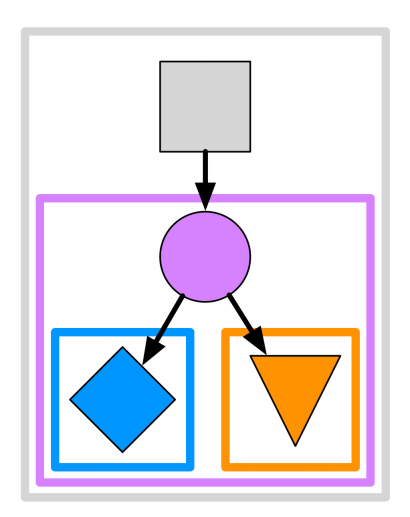
\includegraphics[width=7cm]{chaps/lr/tumor_clone_tree}}
	\caption{درخت کلون تومور}
	\label{fig:ch_lr:tumor_clone_tree}
\end{figure}




\section{تغییرات تعداد کپی }

بیشتر ژنوم انسان دیپلوئید است، به این معنی که دو نسخه از توالی دی‌ان‌ای ما در سلول‌های ما وجود دارد، یکی از پدر و دیگری از مادر. تغییرات شماره کپی این تغییر را می‌دهند، یا با تغییر در تعداد نسخه‌ها (مثلاً از طریق تکثیر کل ژنوم)، نسبت کپی‌های مادر به پدر (مثلاً از دست دادن خنثی هتروزیگوزیته در تعداد کپی‌ها، جایی که برای همان منطقه یک ژنوم والدین تکثیر می‌شود و دیگری حذف شده است) یا هر دو (به عنوان مثال کپی کروموزوم مادر). بیشتر این تغییرات (به استثنای تکثیر کل ژنوم) دامنه محدودی از ژنوم را تحت تأثیر قرار می‌دهد، اما می‌تواند از تأثیر یک ژن تا یک کروموزوم کامل باشد. این بخش از ژنوم تغییر یافته به عنوان یک بخش شناخته می‌شود.


تغییرات شماره کپی می‌توانند تعداد کپی کل یک بخش و / یا تعداد نسبی نسبی دو کروموزوم والدین را تغییر دهند. هر یک از این تغییرات توسط توالی¬یابی ژنومی هسته قابل تشخیص است. تغییر در تعداد کپی کل یک بخش را می‌توان تشخیص داد زیرا نسبت خواندن آن نقشه به آن بخش بین خط جوانه زنی و نمونه تومور متفاوت خواهد بود. بخش از یک قطعه نسبت ورود خوانده شده است که به یک قطعه در یک نمونه غیر سرطانی ترسیم شده است به نسبت خوانده شده که به یک بخش در یک نمونه سرطانی ترسیم شده است. از نسبت نسبت‌ها برای محاسبه این واقعیت استفاده می‌شود که تعداد کل قرائت‌ها اغلب بین توالی یابی سرطانی و غیرسرطانی متفاوت است، در مناطق مختلف ژنوم عمق خواندن بیشتر یا پایین تر ناشی از محتوای \lr{GC} یا نقشه برداری وجود دارد و تردستی یک تومور با بافت طبیعی متفاوت است. تکرر یک ژنوم، میانگین تعداد کپی از هر کروموزوم است که برای طول کروموزوم نرمال می‌شود.


با تغییر در کسر آلل می‌توان عدم تعادل در تعداد نسخه‌های مادری و پدری این بخش را تشخیص داد. در مناطق دیپلوئید ژنوم‌ها، اگر یک بازه بین کپی‌های مادر و پدر متفاوت باشد، موقعیت هتروزیگوت نامیده می‌شود. جهش‌های تک پایه، خط جوانه زنی همچنین به عنوان چند شکلی تک هسته‌ای نامیده می‌شوند. وقتی یک ژنوم توالی یابی شود، حدود نیمی از قرائت آن مکان هتروزیگوت حاوی هر یک از بازها خواهد بود، در نتیجه کسر آلل 50 است. این امر تا زمانی که نسبتی برابر با نسخه‌های مادرانه و پدری وجود داشته باشد، صادق خواهد بود. اگر این نسبت تغییر کند، کسر آلل  تمام پولیمورفیسم تک هسته‌ای در بخش آسیب دیده تغییر می‌کند. پولیمورفیسم تک هسته‌ای هتروزیگوت به طور متوسط هر 1500 باز \cite{chen2012personal} رخ می‌دهد و بنابراین برای بخشهای طولانی بسیاری از پولیمورفیسم تک هسته ایی هتروزیگوت تحت تأثیر قرار می‌گیرند. توزیع کسر آلل \lr{S} تمام پولیمورفیسم تک هسته‌ای در بخش، حالت دوگانه‌ای پیدا می‌کند که هر حالت نشان دهنده نسبت نسخه‌های آن بخش از هر والد است.

فراخوانی \lr{CNA} چالش برانگیز است زیرا با مشاهده مستقل هر بخش، مسئله هنوز مشخص نشده است. حتی با فرض اینکه هر بخش فقط توسط یک \lr{CNA} تحت تأثیر قرار گیرد، \lr{CNA} موسوم به سه پارامتر (نسبت سلولهای حاوی \lr{CNA}، تعداد کپی‌های مادر و تعداد کپی‌های پدری) وجود دارد و فقط دو مشاهده برای توضیح وجود دارد (و کسر آلل )

همه روش‌ها با فرض اینکه تعداد کمی از نژادهای زیرکلونال مسئول بیشتر یا تمام تغییرات شماره کپی هستند، این ابهام را برطرف می‌کنند. روشی که توسط الگوریتم باتنبرگ \cite{nik2012life} به کار رفته است، به بیشتر تغییرات شماره کپی وابسته به یک نژاد زیر کلونال منفرد و شایع به نام تبار کلونال متکی است. تحت این روش، شیوع این تبار، همراه با تعداد کپی اصلی و جزئی در تمام تغییرات تعداد کپیکلونال، می‌تواند با یک فرآیند دو مرحله‌ای تخمین زده شود. در گام اول، این روش با فرض شیوع نژاد کلون $f_c$  آغاز می‌شود. شیوع تبار کلونال در بیشتر موارد با خلوص نمونه تومور برابر است. با توجه به شیوع کلونال، هر بخش پس از آن فقط دو متغیر برای توضیح دارد (تعداد کپی بزرگ و جزئی). از آنجا که هر بخش دارای دو مشاهدات است، اکنون مسئله هنوز به درستی تعیین نشده است و بهترین کپی اصلی و مینور متناسب است. سپس، ترکیب کلی مقدار $\Phi_c$  فرض شده با ترکیب مناسب در تمام بخشها تعیین می‌شود. الگوریتم با بهینه سازی این تناسب بهترین مقدار $\Phi_c$  را انتخاب می‌کند. سپس برای هر بخش، شماره کپی اصلی و جزئی با بهینه سازی متناسب بودن قطعه با بهترین مقدار $\Phi_c$   انتخاب می‌شود. این روش فرض می‌کند که تمام تغییرات شماره کپی به نژاد کلونال تعلق دارند، که همیشه درست نیست. در مرحله بعدی، بخشهایی که حاوی تغییرات تعداد کپیتحت کلونال هستند با جستجوی بخشهایی با اطلاعات مناسب ضعیف با استفاده از $\Phi_c$   استنباط شده مشخص می‌شوند. در این بخش‌ها، روش به طور همزمان و مستقل از هر بخش دیگر، عدد $\Phi_i$   و عدد کپی بزرگ و جزئی را استنباط می‌کند.


از آنجا که سه متغیر وجود دارد و تنها دو مشاهده وجود دارد، راه حل‌های بسیاری با تناسب داده برابر وجود دارد که از نظر زیست شناختی برای این تغییرات تعداد کپی زیر کلونال قابل قبول است. این ابهام با انتخاب راه حلی که نزدیکترین شماره به شماره نسخه طبیعی است برطرف می‌شود، اما تعدادی از موارد متداول وجود دارد که این ابتکار عمل ناموفق است. سپس این روش‌ها انتساب تغییرات تعداد کپی زیرکلونال به دودمان و تمام استنباط‌های فیلوژنتیک را برای روش‌های پایین دست رها می‌کنند.


رویکرد عمده دیگر این است که فرض کنیم همه تغییرات شماره کپی از تعداد کمی تبار ساب کلونال به وجود می‌آیند. الگوریتم هایی که از این روش استفاده می‌کنند به طور مشترک شیوع این نژادها و تعداد کپی بزرگ و جزئی را برای هر بخش استنتاج می‌کنند (به عنوان مثال \lr{THetA}\cite{zhu2011metabolic, vander2009understanding} و \lr{TITAN} ).  تعداد دودمانهای زیر کلونال معمولاً با استفاده از احتمال جریمه شده‌ای مانند معیار اطلاعات بیزی (\lr{BIC}) یا انواع \lr{BIC} تعیین می‌شود (به عنوان مثال \lr{THetA} از \lr{BIC} اصلاح شده با پارامتر مقیاس گذاری استفاده می‌کند \cite{zhu2011metabolic}). بنابراین این روش‌ها هم تغییرات شماره کپیرا فراخوانی می‌کنند و هم آنها را به دودمان‌های زیرکلونال اختصاص می‌دهند. هیچ روش موجود این دودمان‌ها را در یک درخت فیلوژنتیک قرار نمی‌دهد



\section{جهش‌های ساده بدنی }

جهش‌های ساده بدنی‌ جهش‌های كوچكی هستند كه می‌توانند مستقیماً از طریق توالی‌یابی و نسبت كروموزوم‌های موجود در نمونه حاوی آنها از تعداد قرائت‌های حاوی جهش و تعداد كل خوانده‌ها در آن مكان، مشاهده شوند. نسبت قرائت حاوی جهش به کل قرائت به عنوان \lr{VAF} جهش شناخته می‌شود. جهش‌های ساده بدنی‌ها معمولاً با بررسي مشترك ترازها و يك نمونه غير‌سرطاني خوانده مي‌شوند. این استنباط مشترک برای جداسازی انواع بدنی و ژرمینال مورد نیاز است.

این فرایند به دلیل انواع مختلف خطاها و تعصبات که در داده‌های \lr{NGS} وجود دارد، دشوار می‌شود\cite{friedl2010plasticity}. یک مشکل اساسی در تشخیص جهش‌های ساده بدنی‌ این است که به نظر می‌رسد خطاهای توالی جهش‌های ساده بدنی شیوع کمی دارند. به طور خاص، در  \lr{Illumina Hiseq2000}  که به طور گسترده استفاده می‌شود، از هر 1000 پایه یکی از آنها دارای یک خطا است (به طور معمول یک تعویض) \cite{sabeh2009protease}. به همین ترتیب، در طول سه میلیارد پایه ژنوم انسانی، یک احتمال غیر قابل اغماض وجود دارد که در بعضی موقعیت‌ها، چندین بار خواندن دقیقاً شامل خطای توالی دقیقاً در همان موقعیت‌ها است. به نظر می‌رسد این خطاها شیوع کم جهش‌های ساده بدنی دارند. تمایز بین این خطاها و شیوع کم واقعی جهش‌های ساده بدنی‌ها شامل یک معامله بین حساسیت و ویژگی و در حالت ایده آل، یک مدل نویز بسیار دقیق است. حل این مشکل امتداد طبیعی کار گسترده‌ای است که در زمینه فراخوانی جهش‌های جوانه‌زنی انجام شده است و الگوریتم‌های زیادی برای انجام این کار وجود دارد (به عنوان مثال \cite{friedl2010plasticity, demicheli2008effects} )


\section{\gls{allelecdropout}}

اگرچه روش‌های تعیین توالی با بازدهی بالا \cite{hugo2007epithelial} ارزان هستند، اما تحت تاثیر مقدار بایاس هستند و مارکرهای ژنتیکی¬ای تولید می‌کنند که تقریباً به طور تصادفی در کل ژنوم تقسیم می‌شوند. این روشها با موفقیت در \gls{mapping} صفات \cite{nowell1976clonal, greaves2012clonal} ، ساخت مپ پیوندی \cite{sakr1993frequency, fearon1990genetic} ،  اسکن انتخاب  \cite{dentro2018portraits, waclaw2015spatial}،  و برآورد تنوع ژنتیکی \cite{de2006clonal} استفاده شده است. یکی از این روش‌ها، تعیین ژنوتیپ براساس توالی \cite{anderson2011genetic} (\lr{GBS}) است. در \lr{GBS}، هدف توالی یابی فقط با اتصال آداپتورهای توالی به محل‌های برش آنزیم محدود کننده، به کمتر از $5\%$ از ژنوم کاهش می‌یابد (شکل زیر).  قرائت \lr{GBS} همچنین می‌تواند به صورت کانکت‌های کوتاه مونتاژ شود، که بدون نیاز به توالی ژنوم فراخوانی یک نوع تغییر تک هسته‌ای (تغییرات تک نوکلئوتیدی ) را امکان پذیر می‌کند \cite{hanahan2000hallmarks}. از این رو، \lr{GBS} یک روش محبوب در سیستم‌های غیر مدلی است که به طور معمول فاقد منابعی مانند مجموعه ژنوم و ریزآرایه‌ها است.

بر خلاف توالی یابی كل ژنوم \lr{(WGS)} ، \lr{GBS} مستعد ابتلا به خطاهای مختلف تماس به دلیل محدودیت چندشكلی‌های سایت  است (کاهش آللیک). کاهش آللیک در \lr{GBS} می تواند برنامه‌هایی را که به فراخوانی دقیق تغییرات نادر ، از جمله تخمین طیف فرکانس سایت در ژنتیک جمعیت متکی هستند ، را دچار اختلال کند. یک رویکرد آماری سیستماتیک برای تشخیص کاهش آللیک در داده‌های توالی \lr{GBS} ، اجرا شده و  در بسته نرم افزاری منبع باز \lr{GBStools} وجود دارد.  این روش مبتنی بر این واقعیت است که کاهش آللیک متناسب با تعداد آللهای سایت محدود کننده بدون برش که در آنجا حمل می کند ، میزان خوانش نمونه را در یک سایت خاص کاهش می دهد. بنابراین \lr{GBStools} پوشش هر نمونه را در یک سایت خاص به عنوان یک متغیر تصادفی پواسون مورد استفاده قرار می دهد که از توزیع با میانگین \lr{$\lambda$} (آللیک های بدون برش صفر) ، توزیع با میانگین ½\lr{$\lambda$} (یک آللیک بدون برش) ، یا با میانگین صفر (دو آللیک بدون برش). \lr{GBStools} حداکثر احتمال پارامتر \lr{$\lambda$} را با استفاده از تعداد واقعی آللیک های بدون برش در هر نمونه که به عنوان متغیرهای نهفته (مشاهده نشده) در نظر رفته می‌شود و از طریق  حداکثر رساندن  مقدار چشم انتظاری \lr{(EM)}، محاسبه می‌کند . از مقادیر مورد انتظار این متغیرهای نهفته می‌توان برای تخمین اینکه کدام نمونه ها یک آللیک بدون برش دارند استفاده کرد. به طور همزمان ، \lr{GBStools} فرکانس سایت آلل های \lr{SNP} مرجع قابل مشاهده و جایگزین، \lr{$\varphi_1$} و  \lr{$\varphi_2$}   ، و آللیک بدون برش ، \lr{$\varphi_3$}  ، که در آن  \lr{$\varphi_1$+$\varphi_2$+$\varphi_3$=1}   برآورد می کند و در نهایت ، آزمون نسبت احتمال با مقایسه فرضیه صفر  \lr{$\varphi_3$ = 0} با فرضیه \lr{$\varphi_3$> 0} جایگزین می کند. \lr{GBStools}  در اجرای فعلی خود نمی تواند ژنوتیپ های واقعی پنهان شده توسط کاهش آللیک را استنباط کند ، اما می توان با فیلتر کردن سایت هایی که نسبت احتمال آنها زیاد است خطاها را حذف کند.

\begin{figure}[!ht]
	\centerline{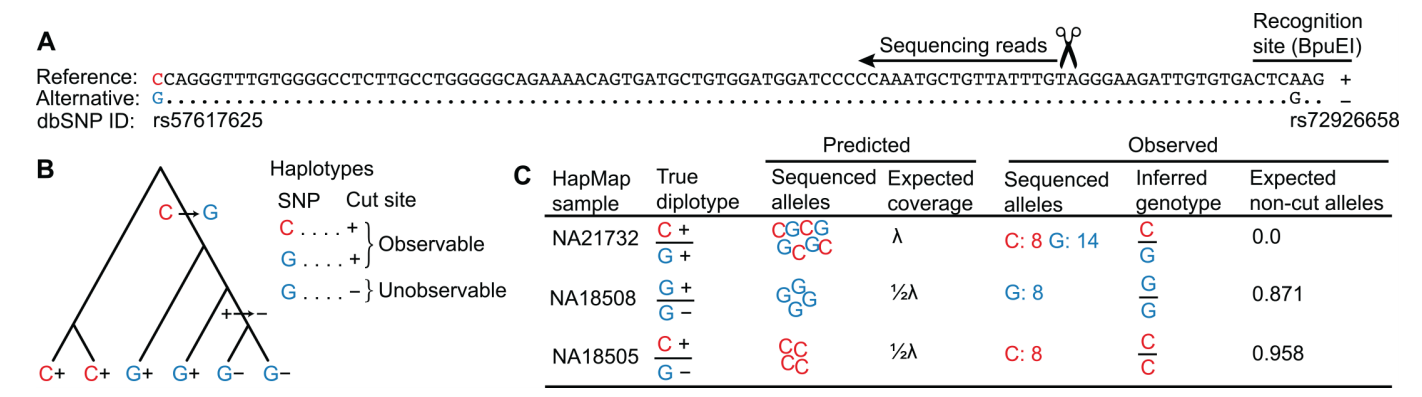
\includegraphics[width=\textwidth]{chaps/lr/mtsd}}
	\caption{نمایی از تطابق ژنتیکی}
	\label{fig:ch_lr:mtsd}
\end{figure}

در شکل بالا، آلل \lr{BpuEI} بدون برش ناشی از \lr{SNP rs72926658} با برچسب "-`` و آلل برش با "+`` برچسب گذاری شده است. آلل "-`` در هاپلوتیپ با آلل \lr{G} مشتق شده بوجود آمده و باعث شده تا برخی از آلل های \lr{G} توسط \lr{GBS} قابل مشاهده نباشند. نمونه های نشان داده شده دارای سه دیپلوتیپ هتروزیگوت است. نتایج توالی با پیش‌بینی‌ها مطابقت داشت و نمونه \lr{NA18505} به اشتباه هموزیگوت نامیده می شد ، اما انتظار می‌رود تعداد آلل‌های کاهشی محاسبه‌شده توسط \lr{GBStools (0.958)} با تعداد واقعی (1) مطابقت داشته باشد، و آن را به عنوان یک تماس اشتباه احتمالی مشخص کند.

\section{مقدمه‌ای بر مدل‌سازی احتمالی }

وظیفه اصلی یادگیری ماشین، یادگیری از داده‌ها است، کاری که به عنوان استنباط شناخته می‌شود. برای یادگیری از داده‌ها، باید فرضیاتی را مطرح کرد. توصیف رسمی فرضیات صورت گرفته به عنوان یک مدل ذکر می‌شود. یک مدل احتمالی مفروضات ارائه شده را تعریف می‌کند که اطلاعات آموخته شده را با استفاده از متغیرهای تصادفی و توزیع‌های احتمال به داده‌های مشاهده شده پیوند می‌دهد. توزیع‌های احتمال توابع ریاضی هستند که یک رویداد را ورودی می¬کنند و احتمال آن واقعه را بیرون می‌آورند. توزیع احتمال می‌تواند تابعی بیش از واقعه باشد و این متغیرهای اضافی به عنوان پارامترهای توزیع شناخته می‌شوند\cite{hanahan2000hallmarks}. 
رویکرد بیزی در یادگیری ماشین شامل استنباط احتمالی مقادیر پارامترهای منوط به مشاهدات است \cite{hanahan2011hallmarks}. چهار مولفه دارد:

\begin{itemize}
	\item 	احتمال: احتمال مشاهده داده‌ها است، مشروط به تنظیم پارامتر \lr{ P(data | parameters)} 
	\item 	پارامترهای احتمال
	\item	پارامترهای قبلی 
	\item داده‌های مشاهده شده
\end{itemize}
پارامترها خود مجموعه‌ای از متغیرهای تصادفی هستند که از توزیع قبلی (\lr{P} (پارامترها)) گرفته شده اند، که باورهای ما را در مورد احتمال حالت‌های مختلف پارامتر در غیاب مشاهده مشاهده می‌کند. این اصطلاحات با استفاده از قانون بیز با هم ترکیب می‌شوند:
\begin{itemize}
	\item \lr{P(parameters|data) = P(data|parameters) $*$ P(parameters) $/$ P(data)}
	\item \lr{Posterior $\propto$ likelihood  $*$  prior}
\end{itemize}
پس زمینه توزیع پارامترهای مشروط به مشاهده داده‌ها است و خروجی اصلی استنتاج بیزی است. از توزیع پسین می‌توان برای انجام کارهایی مانند پیش‌بینی مشاهدات آینده استفاده کرد.


\subsection{\gls{markovchainmontecarlo}}

برای انجام استنتاج \gls{bayesian} ، ما اغلب می‌خواهیم در توزیع پسین ادغام شده، پیش‌بینی کنیم یا خلاصه‌هایی پیدا کنیم، به عنوان مثال میانگین پارامتر پسین. به طور کلی، انجام چنین ادغامی (جمع بندی در مورد متغیرهای گسسته) از نظر تحلیلی غیرقابل حل است. با این حال، می‌توان چنین ادغام هایی را با استفاده از نمونه‌هایی که از قسمت پسین ترسیم شده‌اند تقریبی داد:
\begin{equation}
	E[f]=\int f(x) p(x) d x \approx 1 / N \sum_{1 . . N} f\left(x_{i}\right)
\end{equation}
که در آن $x_i$  نمونه $i$ از $p(x)$ و $p(x)$  و $f(x)$ به ترتیب توزیع و عملکرد مورد نظر ما است. به ندرت می‌توان مستقیماً از توزیع پسین نمونه برداری کرد. برای تولید موثر نمونه‌ها از توزیع، حتی در ابعاد بالا، می‌توان از تکنیک زنجیره ماکوف مونت کارلو استفاده کرد. زنجیره ماکوف مونت کارلو یک زنجیره مارکوف می‌سازد که در آن توزیع تعادل توزیع پسین است. سپس مقادیر زنجیره می‌تواند به عنوان نمونه از پسین با توجه به همگرایی کافی به توزیع تعادل مورد استفاده قرار گیرد. برای انجام زنجیره ماکوف مونت کارلو، تاز زمانی که بتوان \lr{$p \propto p(x)$ } را محاسبه کرد، نیازی به محاسبه $p(x)$  نیست. این زنجیره ماکوف مونت کارلو را قادر می‌سازد تا از محاسبه ثابت‌های نرمال سازی، که اغلب غیرقابل حل هستند، خودداری کند.
یک زنجیره مارکوف به عنوان یک سری متغیرهای تصادفی تعریف می‌شود که دارای ویژگی استقلال شرطی زیر هستند:
\begin{equation}
	p\left(z^{N+1} \mid z^{1} . . z^{N}\right)=p\left(z^{N+1} \mid z^{N}\right)
\end{equation}
نمونه‌ای از الگوریتم زنجیره ماکوف مونت کارلو الگوریتم \lr{Metropolis-Hastings (MH)} است \cite{hastings1970monte}. الگوریتم \lr{MH}  از حالت دلخواه   $Z^t$ شروع می‌شود. سپس یک حالت پیشنهادی $z$  از توزیع پروپوزال \lr{$q(z | z^t)$} ترسیم می‌شود. این حالت پیشنهادی $z$   با احتمال زیر پذیرفته می‌شود:
\begin{equation}
	\min \left(1, \hat{p}\left(z^{*}\right) q\left(z^{t} \mid z^{*}\right) / \hat{p}\left(z^{t}\right) q\left(z^{*} \mid z^{t}\right)\right)
\end{equation}
می توان نشان داد که الگوریتم MH تعادل دقیق را برآورده می‌کند و از این رو،$p(x)$ توزیع تعادل است \cite{bishop2006pattern}. در حالی که توازن دقیق برای اثبات اینکه در محدوده نمونه‌های بی‌نهایت زنجیره به توزیع مورد نظر همگراست کافی است ، اما در عمل فقط تعداد محدودی از نمونه‌ها را می‌توان ترسیم کرد. واضح است که نمونه‌های ابتدای زنجیره ، که از یک مکان دلخواه در فضای حالت شروع می‌شوند ، بعید است از توزیع تعادل باشد. این نمونه‌ها به عنوان نمونه‌های سوختنی کنار گذاشته می‌شوند. هرچه همگرایی زنجیره مارکوف سریعتر باشد، نمونه‌های کمتری باید کنار گذاشته شوند و می‌توان از تعداد بیشتری برای محاسبه انتظارات استفاده کرد. با بررسی اثری از مقادیر مهم پارامتر یا احتمال همگرایی می توان نظارت کرد، اما این امر ممکن است چند حالت را از دست بدهد. متأسفانه دانستن اینکه آیا همگرایی حاصل شده است غیرممکن است، فقط گاهی اوقات می‌توان همگرایی را رد کرد \cite{gelman2011inference}. گذشته از همگرایی ، یکی دیگر از خصوصیات اصلی یک زنجیره مارکوف میزان اختلاط زنجیره است. با توجه به n نمونه مستقل از توزیع ، واریانس میانگین پارامتر برآورد $ \sigma_n $ است که $\sigma$ انحراف استاندارد توزیع خلفی پارامتر است. نمونه‌های گرفته شده از زنجیره مارکوف مستقل نیستند ، زیرا به وضعیت فعلی زنجیره بستگی دارند (یعنی فقط از نظر شرطی مستقل هستند). برای تخمین اندازه نمونه موثر یک زنجیره مارکوف ، یعنی تعداد نمونه‌های مستقل با همان خطای استاندارد همان زنجیره ، می توان از معادله زیر استفاده کرد:
\begin{equation}
	E S S=\frac{n}{1+2 \sum_{0}^{\infty} \rho_{j}}
\end{equation}
حاصل جمع بی نهایت محاسبه \lr{ESS} را می توان با استفاده از برآوردگر پریودوگرام کوتاه تطبیقی \lr{Sokal} \cite{sokal1997monte} تخمین زد.